Durch die intensive Interaktion der Bereiche Entwicklung und Betrieb müssen unterschiedliche organisatorische und kulturelle Veränderungen durchgeführt werden, damit eine DevOps-Kultur etabliert werden kann. In diesem Rahmen baut DevOps auf den Hauptprinzipien \textit{'The Three Ways'} auf, die von Gene Kim einem der Vorreiter des DevOps-Ansatzes \cite{kim_devops-handbuch_2017} definiert wurden. Dieses Model der drei Wege bilden die zugrunde liegenden Prinzipien von DevOps ab, indem das Verhalten und die Muster von DevOps näher beschrieben werden. \cite[S. 9 - 44]{kim_devops-handbuch_2017}, \cite{kim_three_2012}\\\\  

Wie in Abbildung 3 zu erkennen, bildet der erste Weg zunächst die Grundlage für DevOps ab, indem die Leistung des gesamten Systems, im Gegensatz zur der eines einzelnen Teams, Silos oder Abteilungen, in den Vordergrund stellt. Der Fokus liegt auf einem schnellen Arbeitsfluss und Optimierung des gesamten Systems, der durch die IT ermöglicht wird. Das Ergebnis einer lokalen Veränderung zeigt meist keine Wirkung und könnte eine Verschlimmerung der Gesamtsituation herbeiführen. \cite[S. 252]{tiemeyer_handbuch_2021} 

\begin{figure}[h]
    \centering
    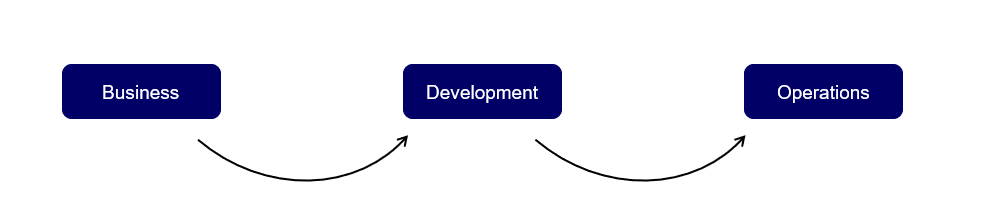
\includegraphics[scale=0.5]{Bilder/First Way.png}
    \caption{Der erste Weg: Systemdenken \cite{kim_three_2012}}
\end{figure}

Den Anfang stellt der Kunde dar, über die Entwicklung bis zu den Operations. Dabei wird das Produkt, basierend auf den identifizierten Kundenanforderungen, von der Entwicklung erstellt und in den Betrieb übergeben, wo das Ergebnis dem Kunden ausgeliefert wird.\cite[S. 12]{halstenberg_devops_2020} Der erste Schritt greift zudem den Grundgedanken des Lean-Ansatzes auf, indem ein Fehler nicht an nachfolgende Arbeitseinheiten weitergegeben werden, damit ein verbesserter Arbeitsfluss aufrecht gehalten werden kann. \cite[S. 252]{tiemeyer_handbuch_2021} Daher sind alle Arbeiten während dieses Schrittes sichtbar und in kleinen Aufgaben aufgeteilt, die in bestimmten Intervallen ausgeführt werden. Zu den Zielen des Ersten Weges gehört, dass bekannte Fehler nicht an nachfolgende Arbeitsplätze weitergegeben werden, damit eine lokale Optimierung nicht zu einer globalen Verschlechterung führt. \cite{kim_three_2012}\\\\  

Gemäß der Abbildung 4, beschreibt der zweite Weg das Gestalten von effizienten Feedbackschleifen, um einerseits Fehler schnell und frühzeitig zu erkennen und zu beheben und andererseits den Prozess durchgängig im Auge zu behalten. Der zweite Schritt stellt den eigentlichen zentralen Ansatzes von DevOps dar, wobei das Feedback von verschiedener Natur sein kann. \cite[S. 254]{tiemeyer_handbuch_2021} 

\begin{figure}[h]
    \centering
    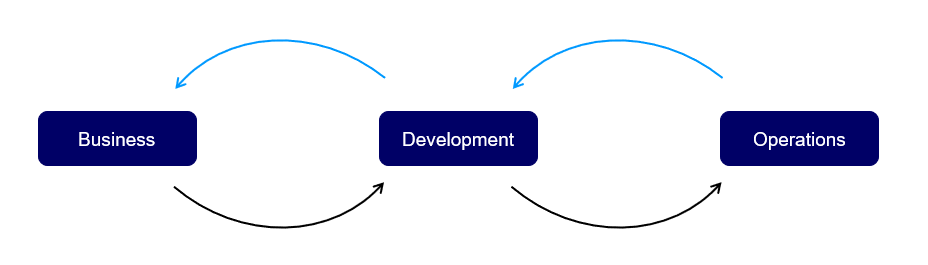
\includegraphics[scale=0.5]{Bilder/Second Way.png}
    \caption{Der zweite Weg: Feedback-Schleifen verstärken \cite{kim_three_2012}}
\end{figure}

Die Feedbackschleifen sollten sowohl auf Seiten von einzelnen Teams untereinander als auch zwischen Entwicklung und Betrieb eingebettet werden. \cite[S. 94]{ravichandran_devops_2016} Je schneller Probleme, Anforderungen oder Auswirkungen kommuniziert werden, desto besser kann verhindert werden, dass Fehler ein zweites Mal auftreten, sich kontinuierlich aufbauen können und sich möglicherweise auf neue Aufgaben auswirken. An dieser Stelle können weitere Kontrollschritte oder schwerfällige Genehmigungsprozesse die Wahrscheinlichkeit für zukünftige Fehler maßgeblich erhöhen. \cite[S. 31]{kim_devops-handbuch_2017} Das Ergebnis des zweiten Wegs stellt die Sicherstellung einer verbesserten Qualität, durch kontniuierliche Feedbackschleifen dar.\\\\ Während der erste Weg technische und der zweite Weg organisatorische Aspekte beinhaltet, zielt der dritte Weg auf die Etablierung kultureller Änderungen ab, um Innovationen weiter voranzutreiben. Anhand der Abbildung 5 zu erkennen, beschreibt der dritte Weg die Schaffung einer Kultur, die einen Ansatz des kontniuierlichen Experimentieres und Lernes ermöglicht. 

\begin{figure}[h]
    \centering
    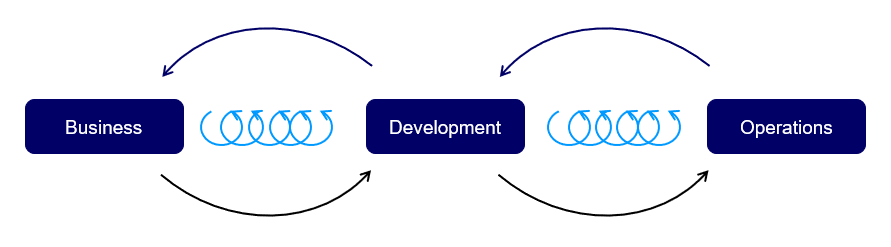
\includegraphics[scale=0.5]{Bilder/Third Way.png}
    \caption{Der dritte Weg: Kultur des kontniuierlichen Experimentierens und Lernens \cite{kim_three_2012}}
\end{figure}

Mittels dieses Weges kann tiefer in die Materie eingegangen werden, um schwierige oder versteckte Probleme identifizieren zu können. Für eine erfolgreiche Durchführung des dritten Weges, sollte die etablierte Kultur auf Vertrauen beruhen. Je höher der Grad des Vertrauens jedes Mitarbeiters, desto wahrscheinlicher und schneller ist die Weitergabe von gewonnenen Erkenntnissen. \cite[S. 357]{kim_phoenix_2014} Infolgedessen sollen Fehler nicht nur aktiv beseitigt, sondern proaktiv danach gesucht und verbessert werden, ohne Kritik auszuüben. \cite[S. 255]{tiemeyer_handbuch_2021} Durch die Möglichkeit der Fehlersuche wird die Motivitation jedes Mitglieds gesteigert und fördert das Experimentieren und daraus ableitende Eingehen eines Risikos, wodurch ein globales Lernen ermöglicht wird. Zu den Ergebnissen des Dritten Weges gehören die Einplanung von Zeit für die Verbesserung der täglichen Abläufe, die Schaffung von Routinen, das Honorieren von eingegangen Risiken und die Einbeziehung von Fehlern in das System, um die Belastbarkeit zu erhöhen.


%Durch die Interaktion der beiden Bereiche Development und Operations gehen auch organisatorische Änderungen mit einher, damit eine umfassende DevOps-Kultur geschaffen werden kann. In diesem Abschnitt wird insbesondere auf die Ziele dieser Kultur eingegangen, damit die Zusammenarbeit zwischen den beiden Bereichen gelingt. In diesem Rahmen wird unter anderem auf die wesentlichen Aspekte/Werte wie Kontniuierliches Lernen, Experimentieren, Ingenieurskultur, Kultur der Effektivität, Produktdenken oder die Übernahme von Verantwortung eingegangen. Auch wird der Vergleich und die Nachteile des traditionellen Silodenkens aufgegriffen. 